% ---------------------
% ARCHITECTURE DU PIPELINE
% ---------------------
\chapter{Architecture du pipeline} \label{ch_three}

\section{Vue d'ensemble et flux de données}

Le pipeline développé dans ce mémoire vise à reconstruire un modèle 3D complet du corps d'un individu à partir d'une vidéo monoculaire d'entraînement, typiquement filmée dans une salle de musculation où l'environnement est encombré (machines, autres individus, miroirs, équipements) et où le sujet est fréquemment partiellement occulté par la barre, les disques, ou les structures de sécurité. Le fait que les vidéos soient captées sans contrôle de la prise de vue, de l'éclairage, ni du fond, impose un enchaînement de modules capables de gérer l'identification du sujet d'intérêt et la complétion d'informations manquantes.

L'architecture proposée est modulaire et séquentielle. Elle s'organise autour de quatre modules principaux fondés sur des modèles de l'état de l'art (SAM3, MoGe-2, TACO, SAM 3D Body), complétés par deux étapes de traitement intermédiaires (filtre de profondeur et isolation du sujet). La figure~\ref{fig:ai-pipeline} en présente la vue d'ensemble.

\begin{figure}[htp]
  \centering
  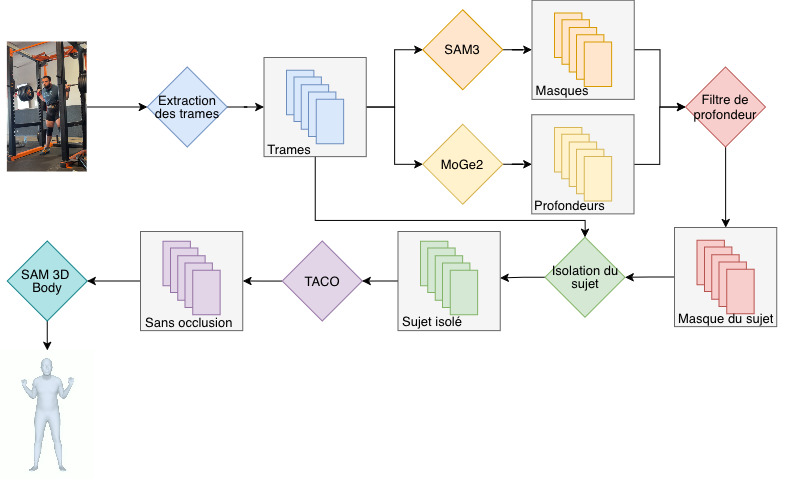
\includegraphics[height=9.5cm]{images/3-Pipeline_architecture/Pipeline.jpg}
  \caption{Vue d'ensemble du pipeline}
  \label{fig:ai-pipeline}
\end{figure}

Le flux de données peut être décrit comme suit :

\begin{enumerate}
  \item La vidéo d'entrée est d'abord décomposée en une séquence d'images individuelles (\textit{trames}).
  \item Deux traitements parallèles sont ensuite appliqués sur chaque image :
  \begin{itemize}
    \item \textbf{SAM3}~\cite{SAM3-2025} génère un ensemble de masques de segmentation correspondant à toutes les personnes présentes dans la scène.
    \item \textbf{MoGe-2}~\cite{MoGe2-2025} produit une carte de profondeur, attribuant à chaque pixel une estimation de sa distance par rapport à la caméra.
  \end{itemize}
  \item Un \textbf{filtre de profondeur} fusionne ces deux sorties pour ne conserver que les masques correspondants au sujet situé au premier plan, écartant ainsi les autres personnes situées en arrière-plan.
  \item L'étape d'\textbf{isolation du sujet} applique ces masques filtrés sur les images originales, produisant une séquence où seul le sujet apparaît sur un fond neutre (blanc).
  \item Ces images sont ensuite traitées par \textbf{TACO}~\cite{TACO-2025}, un modèle de complétion amodale vidéo qui reconstruit les parties du sujet occultées par les équipements (barres, disques, machines), tout en garantissant la cohérence temporelle entre les trames.
  \item Enfin, \textbf{SAM 3D Body}~\cite{SAM-3D-Body-2026} reçoit en entrée la séquence d'images ne présentant plus d'occlusions et reconstruit la pose ainsi que la forme corporelle caractérisant la morphologie de l'individu.
\end{enumerate}

Ce choix d'architecture séquentielle est motivé par plusieurs considérations. D'une part, bien que des approches unifiées telles qu'OpenPose~\cite{OpenPose-2019} ou ViTPose~\cite{ViTPose-2022} permettent d'estimer un squelette 3D et présentent une certaine robustesse aux occlusions partielles, elles demeurent insuffisantes dans notre contexte pour deux raisons. Premièrement, leur robustesse aux occlusions se dégradent face aux occlusions massives et prolongées (voir section~\ref{sec:2d-3d-estimation}), ces occlusions sont caractéristiques des vidéos de force athlétique. Deuxièmement, aucun modèle unique disponible publiquement ne couvre conjointement l'intégralité de la chaîne de traitement requise : isolation du sujet dans un environnement encombré, estimation de profondeur, complétion amodale temporellement cohérente et reconstruction d'un maillage corporel complet. D'autre part, le découpage modulaire permet de remplacer indépendamment chaque composant lorsque de nouveaux modèles plus performants émergent, un point particulièrement pertinent compte tenu du rythme actuel des publications dans le domaine de la vision par ordinateur. Enfin, cette structure offre une meilleure interprétabilité du système, en cas d'erreur en sortie, il est possible d'identifier précisément le module posant problème.

\section{Module 1 : Segmentation avec SAM3} \label{sec:module-1}

\subsection{Principe et architecture}

SAM3 (\textit{Segment Anything Model 3}), publié par Meta en novembre 2025~\cite{SAM3-2025}, est un modèle de segmentation fondationnel introduisant la notion de \textit{Promptable Concept Segmentation} (PCS). Pour comprendre l'apport de SAM3, il est important de rappeler le fonctionnement de ses prédécesseurs. SAM et SAM2 opèrent à partir d'un prompt interactif localisé (un point, une boîte englobante ou un masque grossier) et produisent un unique masque correspondant à l'objet pointé. L'utilisateur  doit donc interagir manuellement avec chaque instance qu'il souhaite segmenter. SAM3 n'utilise plus seulement ce paradigme mais introduit la notion de prompt textuel. Plutôt que de pointer un objet précis, l'utilisateur spécifie une catégorie (par exemple \emph{"human"}) via un prompt textuel. Le modèle détecte alors automatiquement toutes les instances correspondant à ce prompt dans l'image ou la vidéo, et génère un masque pour chacune d'elles, sans intervention manuelle. Dans le pipeline, cette propriété est exploitée pour isoler l'ensemble des personnes présentes dans la scène en une seule inférence, le filtre de profondeur permettra ensuite de sélectionner le sujet d'intérêt au premier plan.

L'architecture repose sur un transformeur double encodeur-décodeur \footnote{Un transformeur double encodeur-décodeur désigne une architecture composée de deux branches parallèles : un encodeur qui extrait des représentations sémantiques de haut niveau depuis l'image d'entrée, et un décodeur qui reconstruit progressivement la sortie depuis ces représentations. Le qualificatif \textit{double} indique que l'architecture dispose de deux paires encodeur-décodeur spécialisées.}. Plus précisément, elle découple un détecteur de type DETR (\textit{DEtection TRansformer}) d'un suiveur vidéo dérivé de SAM2, auquel s'ajoute une "\textit{presence head}" destinée à stabiliser le suivi d'instance sur de longues séquences. Le modèle a été entraîné sur le jeu de données (\textit{dataset}) SA-Co~\cite{SAM3-SA-Co-2025} qui est un dataset de référence pour la segmentation d'objets dans les images, cet ensemble de données contient des images associées à des étiquettes textuelles. SAM3 a atteint une précision moyenne pour des masques de segmentation \textit{zero-shot} de 47.0 mAP (\textit{mean Average Precision}) \footnote{"mean Average Precision" est une métrique globale de la performance d'un modèle de détection d'objets, prenant en compte la précision pour chaque classe d'objet présente dans les prédictions, elle s'exprime sur une échelle allant de 0 à 1 (ou 0\% à 100\%).} sur LVIS~\cite{LVIS-Dataset-2019}, qui est un dataset de référence pour la détection d'objets, contre 38.5 mAP pour le précédent état de l'art. 


\subsection{Entrées et sorties dans le pipeline}

Dans le pipeline, SAM3 est appliqué trame par trame avec un prompt textuel orienté vers la détection de toutes les personnes. Pour chaque trame, SAM3 produit un ensemble de masques binaires correspondant aux personnes détectées, la trame étant traitée indépendamment des trames voisines. Le tracker vidéo intégré à SAM3, bien que disponible, n'est pas exploité dans l'implémentation effectuée en raison de la mémoire GPU requise pour maintenir l'état de tracking sur des séquences longues, incompatible avec la contrainte d'inférence sur les GPU mis à disposition durant le mémoire (voir section~\ref{sec:integration}).

Ce traitement indépendant trame par trame implique que les identifiants d'instance produits par SAM3 ne sont pas cohérents temporellement, le masque associé au sujet à la trame $t$ peut porter l'indice $i$ et celui correspondant au même sujet à la trame $t+1$ porter un indice $j \neq i$. La continuité d'identité est rétablie par la suite via le filtre de profondeur (section~\ref{sec:filtre-profondeur}), qui filtre à chaque trame le masque de la personne la plus proche. Cette stratégie est robuste tant que le sujet d'intérêt reste le plus proche de la caméra, hypothèse vérifiée dans la quasi-totalité des contextes de musculation où l'individu est filmé en premier plan, les autres pratiquants étant systématiquement plus éloignés de la caméra.

\subsection{Justification du choix}

Deux propriétés ont motivé le choix de SAM3 sur d'autres modèles de segmentation candidats (Mask R-CNN~\cite{Mask-R-CNN-2018}, DETR~\cite{DETR-2020}, YOLOv11-seg~\cite{Ultralytics-YOLO-2026}, SAM2~\cite{SAM2-2024}) :

\begin{itemize}
  \item \textbf{Robustesse \textit{zero-shot}.} L'environnement d'une salle de musculation contient des objets atypiques (machines spécifiques, vêtements de sport variés, équipements rares) qui ne figurent pas systématiquement dans les jeux de données classiques. La capacité de SAM3 à généraliser sans fine-tuning évite une coûteuse et longue phase de réannotation.
  \item \textbf{Promptabilité conceptuelle.} La possibilité de cibler explicitement le concept \emph{"personne"} par simple texte simplifie considérablement l'intégration dans le pipeline.
\end{itemize}

\subsection{Limites et alternatives}

SAM3 présente toutefois plusieurs limites dans notre contexte. Premièrement, la latence d'inférence reste élevée sur du matériel local : alors que les auteurs rapportent environ 30 ms par image sur GPU H200, le temps d'inférence observé sur notre configuration (NVIDIA RTX
A5000, 24 Go GDDR6) est nettement supérieur (environ 200 ms, mesuré expérimentalement sur la station de travail) en raison de la moindre puissance de calcul de la RTX A5000 par rapport au GPU H200 utilisé par les auteurs. Ce point exclut toute exécution en temps réel sur ce matériel et impose un traitement en post-production. Deuxièmement, le modèle peut produire des masques fragmentés lorsque le sujet est partiellement occulté par un objet de couleur similaire (par exemple un t-shirt noir devant un fond noir), nécessitant un post-traitement morphologique (fermeture suivie d'une sélection de la composante connexe principale). Troisièmement, en cas de présence de plusieurs personnes proches dans le champ, la sélection automatique du sujet d'intérêt requiert le filtre de profondeur décrit en section~\ref{sec:filtre-profondeur}. Enfin, l'absence d'exploitation du tracker vidéo intégré (justifiée précédement) impose de reconstruire la continuité d'identité par la suite, ce qui peut occasionnellement échouer lorsque par exemple deux personnes se croisent à des profondeurs similaires.

Des alternatives ont été considérées et écartées :
\begin{itemize}
  \item \textbf{SAM2} fournit une excellente segmentation interactive mais ne permet pas de détecter spontanément toutes les instances d'un concept par prompt textuel.
  \item \textbf{Grounded-SAM} combine GroundingDINO et SAM en deux passes séquentielles (détection textuelle puis segmentation) ce qui double le temps d'inférence par rapport à un modèle unifié.
  \item \textbf{YOLOv11-seg} offre une latence très faible mais ses masques sont moins précis que SAM3. Cette imprécision dégraderait la précision du filtre de profondeur, qui calcule la profondeur du sujet sur la base de son masque. Un masque grossier inclurait des pixels d'arrière-plan proches du sujet, biaisant l'estimation lorsque plusieurs personnes apparaissent à des profondeurs comparables.
\end{itemize}

\section{Module 2 : Carte de profondeur avec MoGe-2} \label{sec:module-2}

\subsection{Principe et architecture}

MoGe-2 (\emph{Monocular Geometry estimation v2}) est un modèle d'estimation de géométrie monoculaire publié en 2025 par Microsoft~\cite{MoGe2-2025}. Là où l'estimation de profondeur classique se limite à prédire un scalaire par pixel, MoGe-2 prédit directement un \emph{point map} 3D métrique, c'est-à-dire l'association de chaque pixel à un point $(X, Y, Z)$ exprimé dans un repère avec une échelle réelle.

MoGe-2 repose sur une architecture de type encodeur-décodeur fondée sur un transformeur de vision (\textit{Vision Transformer}) pré-entraîné. Le modèle a été entraîné sur un corpus hétérogène massif combinant des données réelles issues de scanners LiDAR \footnote{Le LiDAR (\emph{Light Detection And Ranging}) est un capteur qui mesure la distance par rapport aux objets en émettant des impulsions laser et en mesurant le temps de retour de l'écho. Il produit un nuage de points 3D dense, constituant une vérité terrain de profondeur précise au centimètre.} et de capteurs RGB-D\footnote{Un capteur RGB-D (Red Green Blue - Depth) est un dispositif combinant une caméra couleur standard et un capteur de profondeur (typiquement infrarouge). Il produit simultanément une image couleur et une carte de profondeur alignée pixel à pixel, fournissant ainsi une représentation 2,5D de la scène.}, des données synthétiques générées par rendu 3D, ainsi que des pseudo-vérités terrain produites par des méthodes de reconstruction multi-vues. Cette diversité des sources d'entraînement est la clé de sa capacité de généralisation \textit{zero-shot} : des estimations métriques cohérentes sont produites sur des images non vues lors de l'entraînement, sans calibration préalable de la caméra. Dans le pipeline présenté dans ce mémoire, cette propriété est exploitée pour stratifier spatialement la scène et isoler l'athlète au premier plan par un filtre de profondeur.

L'architecture combine deux innovations majeures par rapport au modèle original MoGe :

\begin{enumerate}
  \item Une représentation hybride associant un point map (héritage de MoGe) à un facteur d'échelle global~\cite{MoGe-2025}, ils sont prédits séparément, ce découplage permet de bénéficier de la qualité géométrique offerte par la prédiction tout en récupérant l'échelle métrique réelle, contournant ainsi l'ambiguïté focale-distance \footnote{En vision monoculaire, la distance d'un objet à la caméra et la longueur focale de l'objectif produisent des effets sur la projection 2D : un objet lointain capturé avec un téléobjectif produit la même image qu'un objet proche capturé avec un grand-angle. Sans connaissance préalable de la focale, il est donc impossible de récupérer l'échelle métrique absolue depuis une seule image.}.
  \item Une stratégie de raffinage des données d'entraînement (\textit{data refinement}) qui filtre et complète les annotations bruitées des jeux de données réels en s'appuyant sur des labels synthétiques. Cette procédure améliore significativement la finesse des contours sans dégrader la précision globale.
\end{enumerate}

Le modèle prédit aussi le point map, la profondeur dérivée et le champ de vision (\textit{FOV}) de la caméra, ce qui est particulièrement utile dans un contexte où les métadonnées de capture sont souvent indisponibles, comme c'est le cas pour les vidéos d'entraînement filmées par des pratiquants amateurs.

\subsection{Entrées et sorties dans le pipeline}

MoGe-2 est appliqué indépendamment à chaque trame et produit une carte de profondeur métrique. À chaque pixel est associée une distance exprimée en mètres. Cette carte est ensuite passée au filtre de profondeur (section~\ref{sec:filtre-profondeur}) pour identifier les pixels appartenant au sujet de premier plan. Le seuil de séparation entre premier plan et arrière-plan n'est pas fixé manuellement : il est estimé automatiquement à partir de la distribution des profondeurs dans la carte, en identifiant le pic de profondeur minimal correspondant au sujet le plus proche de la caméra. Cette approche adaptive dispense de toute calibration préalable et reste valide quelle que soit la distance entre l'athlète et la caméra.

\subsection{Justification du choix}

Plusieurs modèles de profondeur monoculaire étaient candidats : MiDaS~\cite{MiDaS-2020}, ZoeDepth~\cite{ZoeDepth-2023}, Depth Anything V2~\cite{Depth-Anything-V2-2024}, Marigold~\cite{Marigold-2024}, UniDepth~\cite{UniDepth-2024}, et MoGe-2~\cite{MoGe2-2025}. Le choix s'est porté sur MoGe-2 pour les raisons suivantes :

\begin{itemize}
  \item \textbf{Échelle métrique native.} Contrairement à MiDaS ou Depth Anything qui produisent une profondeur relative, MoGe-2 fournit directement des valeurs métriques exploitables pour le filtrage spatial.
  \item \textbf{Précision sur les contours.} La stratégie de raffinement des données conduit à des silhouettes humaines nettement plus précises que les concurrents~\cite{MoGe2-2025}, ce qui est important pour éviter qu'un pixel du sujet ne soit attribué au fond (ou inversement) lors de la combinaison avec les masques SAM3.
  \item \textbf{Robustesse open-domain.} Le modèle a été entraîné sur un corpus de 24 jeux de données~\cite{MoGe2-2025} totalisant environ 8,9 millions de trames, combinant trois types de sources : des données réelles issues de scanners LiDAR, des reconstructions SfM (\textit{Structure from Motion})\footnote{La reconstruction \emph{Structure from Motion} (SfM) est une technique de vision par ordinateur permettant de reconstruire une scène 3D et la trajectoire de la caméra à partir d'un ensemble d'images 2D prises sous différents angles.} en environnements intérieurs comme extérieurs, et des données synthétiques. Cette diversité garantit une généralisation robuste à des environnements non vus lors de l'entraînement, comme les salles de sport.
\end{itemize}

\subsection{Limites et alternatives} \label{subsec:background-limitation}

Dans les salles de musculation fréquentées, d'autres individus peuvent apparaître dans le champ de la caméra. Lorsque leurs vêtements présentent une couleur ou une luminosité similaire à ceux du sujet d'intérêt, le filtre de profondeur peut échouer à les différencier correctement. La figure~\ref{fig:background-limitation} illustre ce cas : un second pratiquant en tenue claire, visible en arrière-plan, est partiellement fusionné avec la main du sujet principal dans le masque produit par SAM3. Le filtre de profondeur, qui s'appuie sur la profondeur médiane du masque pour identifier le sujet au premier plan, est mis en échec lorsque les deux silhouettes se chevauchent visuellement à des profondeurs pourtant distinctes. La reconstruction TACO reçoit alors une silhouette étendue incluant des pixels appartenant à l'autre pratiquant, introduisant des artefacts dans les régions concernées.

\begin{figure}[htp]
  \centering
  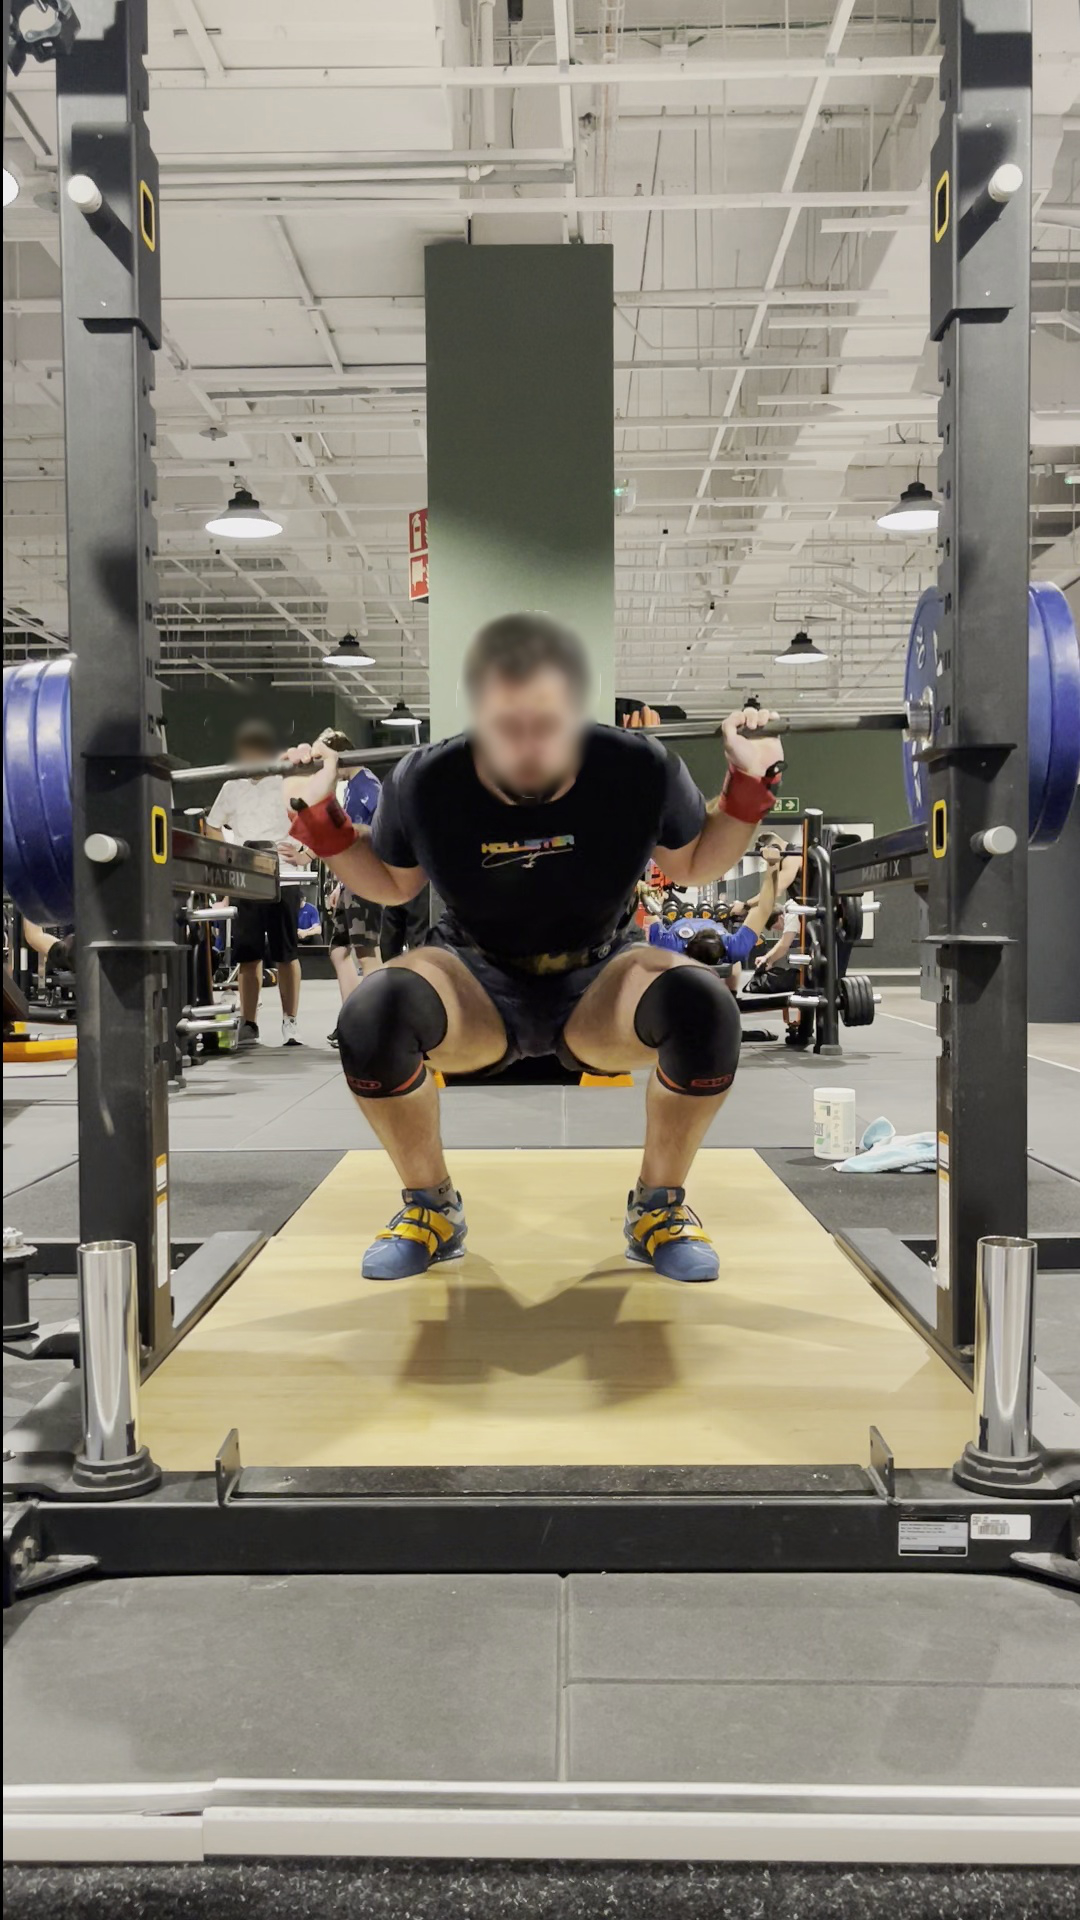
\includegraphics[width=3cm, height=5cm]{images/3-Pipeline_architecture/Background-limitation-frame.jpg}
  
\includegraphics[width=3cm, height=5cm]{images/3-Pipeline_architecture/Background-limitation-moge.png}
  
\includegraphics[width=3cm, height=5cm]{images/3-Pipeline_architecture/Background-limitation-mask.png}
  \caption{Confusion entre sujet et fond de couleur similaire}
  \label{fig:background-limitation}
\end{figure}

La principale limite de MoGe-2 dans notre cas est la suivante : la prédiction d'échelle métrique reste sujette à des erreurs de l'ordre de 5 à 10\,\% en environnements très inhabituels~\cite{MoGe2-2025} (très faible éclairage, scènes monochromes, ...), ce qui peut affecter la stabilité du filtre de profondeur.

Une alternative pertinente était UniDepth~\cite{UniDepth-2024}, qui fournit également des prédictions métriques. Il a été écarté en raison d'une qualité de contour inférieure. Depth Anything V2~\cite{Depth-Anything-V2-2024}, malgré son excellente généralisation, a été éliminé pour son absence d'échelle métrique native et sa précison inférieure à MoGe-2~\cite{Depth-Anything-V2-2024}.

\section{Filtre de profondeur et isolation du sujet} \label{sec:filtre-profondeur}

Ces deux étapes intermédiaires, bien que n'utilisant pas de modèle profond, jouent un rôle important dans le pipeline.

\subsection{Filtre de profondeur}

Le filtre de profondeur reçoit en entrée l'ensemble des masques produits par le module 1 (voir section~\ref{sec:module-1}) et la carte de profondeur produite par le module 2 (voir section~\ref{sec:module-2}) pour une trame donnée. Son objectif est d'identifier, parmi tous les masques détectés, celui correspondant au sujet d'intérêt situé au premier plan.

Pour chaque masque, la profondeur médiane des pixels couverts est calculée. Le masque retenu est celui présentant la plus faible profondeur parmi les personnes détectées.

\subsection{Isolation du sujet}

Une fois le masque du sujet identifié, l'isolation consiste simplement à appliquer ce masque sur l'image originale, produisant une séquence d'images où seul le sujet apparaît sur un fond neutre (blanc).

Cette étape remplit deux rôles distincts dans le pipeline. D'une part, elle simplifie radicalement le problème posé aux modules suivants : en supprimant toute personne autre que le sujet d'intérêt, TACO et SAM 3D Body n'ont plus à gérer la présence d'autres pratiquants dans le champ, ce qui évite les confusions d'instance et les reconstructions erronées dues à une silhouette parasite (voir sous-section~\ref{subsec:background-limitation}). D'autre part, elle élimine les biais visuels introduits par l'arrière-plan d'une salle de musculation : miroirs multipliant les instances apparentes du sujet, reflets sur les équipements métalliques, et présence de couleurs similaires à celles de l'habillement de l'athlète dans le fond de la scène (voir sous-section~\ref{subsec:background-limitation}).


\section{Module 3 : Complétion amodale d'occlusions avec TACO} \label{sec:module-3}

\subsection{Principe et architecture}

TACO (\emph{Taming Diffusion for in-the-wild Video Amodal Completion})~\cite{TACO-2025}, publié en 2025, est un modèle de diffusion conditionnel\footnote{Un modèle de diffusion conditionnel est une extension des modèles de diffusion génératifs dans laquelle le processus de débruitage est guidé par un signal de conditionnement externe (image, masque, texte, etc.). Plutôt que de générer des données depuis du bruit pur de manière inconditionnelle, le modèle apprend à produire des sorties cohérentes avec la condition fournie.} dédié à la tâche de \emph{Video Amodal Completion} (VAC). TACO réutilise les variétés \footnote{En apprentissage automatique, une variété (\textit{manifold}) désigne une structure géométrique de basse dimension apprise par le modèle dans l'espace des données. Un modèle de diffusion pré-entraîné apprend implicitement la variété des vidéos naturelles, c'est-à-dire la distribution des apparences et mouvements plausibles.} apprises par un modèle de diffusion vidéo pré-entraîné (\textit{Stable Video Diffusion}, SVD~\cite{SVD-2023}) et les adapte au problème de VAC via un fine-tuning. Le modèle reçoit en entrée une séquence vidéo (\textit{trames}) dans laquelle un objet d'intérêt est partiellement occulté, ainsi que son masque visible. Il produit une séquence vidéo dans laquelle l'objet est entièrement reconstruit, y compris les parties précédemment cachées, avec une cohérence temporelle assurée par la nature vidéo du modèle de diffusion sous-jacent.

L'apprentissage repose sur le dataset synthétique OvO (\emph{Object-video-Overlay})~\cite{TACO-2025}, construit en superposant artificiellement des occlusions synthétiques sur des vidéos non-occultées. Ce dataset est organisé en deux niveaux de difficulté (OvO-Easy et OvO-Hard), et le fine-tuning est conduit progressivement du plus simple au plus complexe.

\subsection{Entrées et sorties dans le pipeline}

Dans le pipeline, TACO reçoit en entrée la séquence d'images isolées ainsi que le masque correspondant au sujet. Sa sortie est une séquence dans laquelle les portions du corps de l'athlète masquées par la barre, les disques ou les structures de sécurité sont reconstruites de façon vraisemblable et temporellement stable.

Ce module est crucial dans le contexte de la force athlétique, lors d'un squat par exemple, les disques ou la structure de sécurité cachent une partie du bras ou de la jambe, et un modèle de reconstruction 3D appliqué directement sur les images occultées produirait des artefacts importants (certaines parties du corps à des positions éronnées).

\subsection{Justification du choix}

Le choix de TACO repose sur trois arguments :

\begin{itemize}
  \item \textbf{Cohérence temporelle.} Contrairement aux méthodes de complétion amodale image par image, TACO exploite explicitement le contexte temporel via le modèle de diffusion vidéo sous-jacent (\textit{Stable Video Diffusion})~\cite{TACO-2025}, évitant le scintillement inter-trames qui dégraderait la reconstruction 3D ultérieure.
  \item \textbf{Capacité en conditions réelles.} TACO a été spécifiquement conçu et évalué pour gérer des vidéos non contraintes, sans hypothèses fortes sur le contexte de capture~\cite{TACO-2025}. Les auteurs rapportent des performances robustes sur des séquences issues d'environnements très variés, ce qui est déterminant dans le contexte d'une salle de musculation.
  \item \textbf{Adaptabilité par fine-tuning.} Le code source de TACO est publié avec des scripts d'entraînement et de fine-tuning directement utilisables~\cite{TACO-2025}. Cette accessibilité ouvre la voie à une spécialisation du modèle sur des données propres au domaine de la force athlétique, comme décrit au chapitre~\ref{ch_four}.
\end{itemize}

\subsection{Limites et alternatives}

TACO présente plusieurs limitations notables. Premièrement, le coût computationnel est élevé, étant basé sur un modèle de diffusion vidéo, il requiert plusieurs secondes d'inférence par séquence sur des GPU haut de gamme, ce qui exclut, ici aussi, tout traitement en temps réel. Deuxièmement, la qualité de la complétion amodale se dégrade lorsque les occlusions couvrent plus de 50\,\% du sujet sur une durée prolongée. Troisièmement, le modèle n'est pas spécialisé sur l'anatomie humaine et peut produire des reconstructions plausibles mais anatomiquement incorrectes (par exemple un coude présentant une flexion irréaliste).

Des alternatives ont été considérées et écartées :
\begin{itemize}
  \item \textbf{pix2gestalt}~\cite{pix2gestalt-2024} effectue une complétion amodale image par image en s'appuyant sur Stable Diffusion. Sans modélisation du contexte temporel, il produit des sorties incohérentes d'une trame à l'autre, ce qui dégrade significativement la qualité de la reconstruction 3D ultérieure.
  \item \textbf{InpaintHuman}~\cite{InpaintHuman-2026} est spécialisé sur l'humain et donc garantit une cohérence anatomique supérieure. Cependant, son intégration nécessite une estimation de pose préalable précise, créant une dépendance circulaire avec le module SAM 3D Body situé en aval de TACO dans le pipeline. Cette contrainte d'ordonnancement a conduit à écarter cette solution.
  \item \textbf{Video inpainting classique}~\cite{ProPainter-2023} atteint d'excellents résultats sur la complétion amodale vidéo, mais ces méthodes requièrent la spécification explicite des masques d'occlusion trame par trame. Or, dans notre cas, identifier automatiquement quelles régions du sujet sont occultées constitue un problème en soi, que TACO résout via la complétion amodale.
  \item \textbf{Diffusion Handles}~\cite{DiffusionHandles-2023} et autres approches de complétion amodale image par image basées sur diffusion souffrent du même défaut que pix2gestalt et ont été écartées pour la même raison.
\end{itemize}


\section{Module 4 : Éstimation de pose avec SAM 3D Body}

\subsection{Principe et architecture}

SAM 3D Body (3DB), publié par Meta en novembre 2025~\cite{SAM-3D-Body-2026}, est un modèle promptable dédié au \emph{Human Mesh Recovery} (HMR)\footnote{\emph{Human Mesh Recovery} désigne la tâche consistant à reconstruire le maillage 3D complet du corps humain (forme corporelle) depuis une ou plusieurs images 2D. Contrairement à l'estimation de pose squelettique qui produit un ensemble discret de keypoints, le HMR produit un maillage dense de plusieurs milliers d'éléments représentant la surface corporelle, incluant la forme du corps (morphologie, corpulence) et la pose (angles articulaires).} à partir d'une image unique. Il atteint l'état de l'art sur plusieurs benchmarks~\cite{SAM-3D-Body-2026} et est conçu pour produire des reconstructions robustes en conditions réelles (\textit{in-the-wild}).

SAM 3D Body repose sur une architecture de type encodeur-décodeur. L'encodeur image adopte une conception multi-entrées capable de capturer des détails à haute résolution pour les parties fines du corps (mains, pieds, visage). Le décodeur prédit les paramètres d'une représentation paramétrique de maillage : la \emph{Momentum Human Rig} (MHR) \footnote{MHR est une représentation paramétrique du corps humain introduite par Meta~\cite{MHR-2025}. Elle encode le corps via deux composantes découplées : un \textit{skeletal rig} définissant la structure articulaire et les rotations osseuses, et une \textit{soft tissue shape} décrivant la forme de la surface cutanée indépendamment de la pose. Ce découplage explicite contraste avec SMPL et SMPL-X, où la forme et la pose sont entremêlées.}. Cette représentation, ouverte et nouvellement introduite par les auteurs, présente la propriété originale de découpler explicitement la structure squelettique (\textit{skeletal rig}) de la forme de la surface (\textit{soft tissue shape}), offrant ainsi une interprétabilité supérieure comparé à SMPL ou SMPL-X.

Le modèle est promptable, il accepte en entrée des masques de segmentation et/ou des keypoints 2D, ce qui permet de guider la reconstruction. Cette propriété n'est pas exploitée dans le pipeline puisque la silhouette sortante de TACO est seule sur un fond uni.

\subsection{Entrées et sorties dans le pipeline}

SAM 3D Body est appliqué trame par trame sur les images produites par TACO. Sa sortie pour chaque trame est un ensemble de paramètres MHR comprenant :
\begin{itemize}
  \item la pose globale du sujet.
  \item les angles articulaires de l'ensemble du squelette, incluant 70 keypoints corps, mains et pieds.
  \item les paramètres de la forme corporelle (\emph{shape parameters}) caractérisant la morphologie du sujet.
\end{itemize}

Ces paramètres permettent de produire un maillage 3D du sujet, qui constitue la sortie finale du pipeline.

\subsection*{Interface de visualisation des résultats}

Une application web de visualisation (figure~\ref{fig:web-visualisation}) a été développée dans le cadre de ce travail de fin d'études pour explorer les reconstructions 3D produites par SAM 3D Body (voir annexe~\ref{ann:web-interface}). Elle permet de naviguer trame par trame dans la séquence reconstruite et affiche en temps réel les métriques biomécaniques calculées à partir des keypoints 3D exportés.

Pour chaque mouvement, des métriques spécifiques aux critères techniques de l'IPF~\cite{IPF-Technical-Regulations-2025} sont calculées à partir des fichiers de keypoints au chargement de la séquence :

\begin{itemize}
  \item \textbf{Squat.} Profondeur de la descente (hanche sous le niveau du genou sur au moins une trame), inclinaison maximale du buste, et asymétrie maximale des hanches sur l'ensemble de la séquence.
  \item \textbf{Développé couché.} Verrouillage des coudes (angle > 160° atteint en fin de mouvement), angle minimal des coudes (profondeur de la descente), et symétrie des poignets.
  \item \textbf{Soulevé de terre.} Verrouillage des genoux, épaules en arrière en position finale, inclinaison maximale du buste, et distance cumulée parcourue par chaque main sur l'ensemble du mouvement.
\end{itemize}

Les métriques globales sont calculées sur l'ensemble de la séquence dès le chargement, tandis que les métriques instantanées (angles courants, symétrie) sont mises à jour à chaque trame. Cette distinction permet à l'entraîneur de distinguer la conformité globale du mouvement de l'état postural à un instant précis.

\begin{figure}[htp]
  \centering
  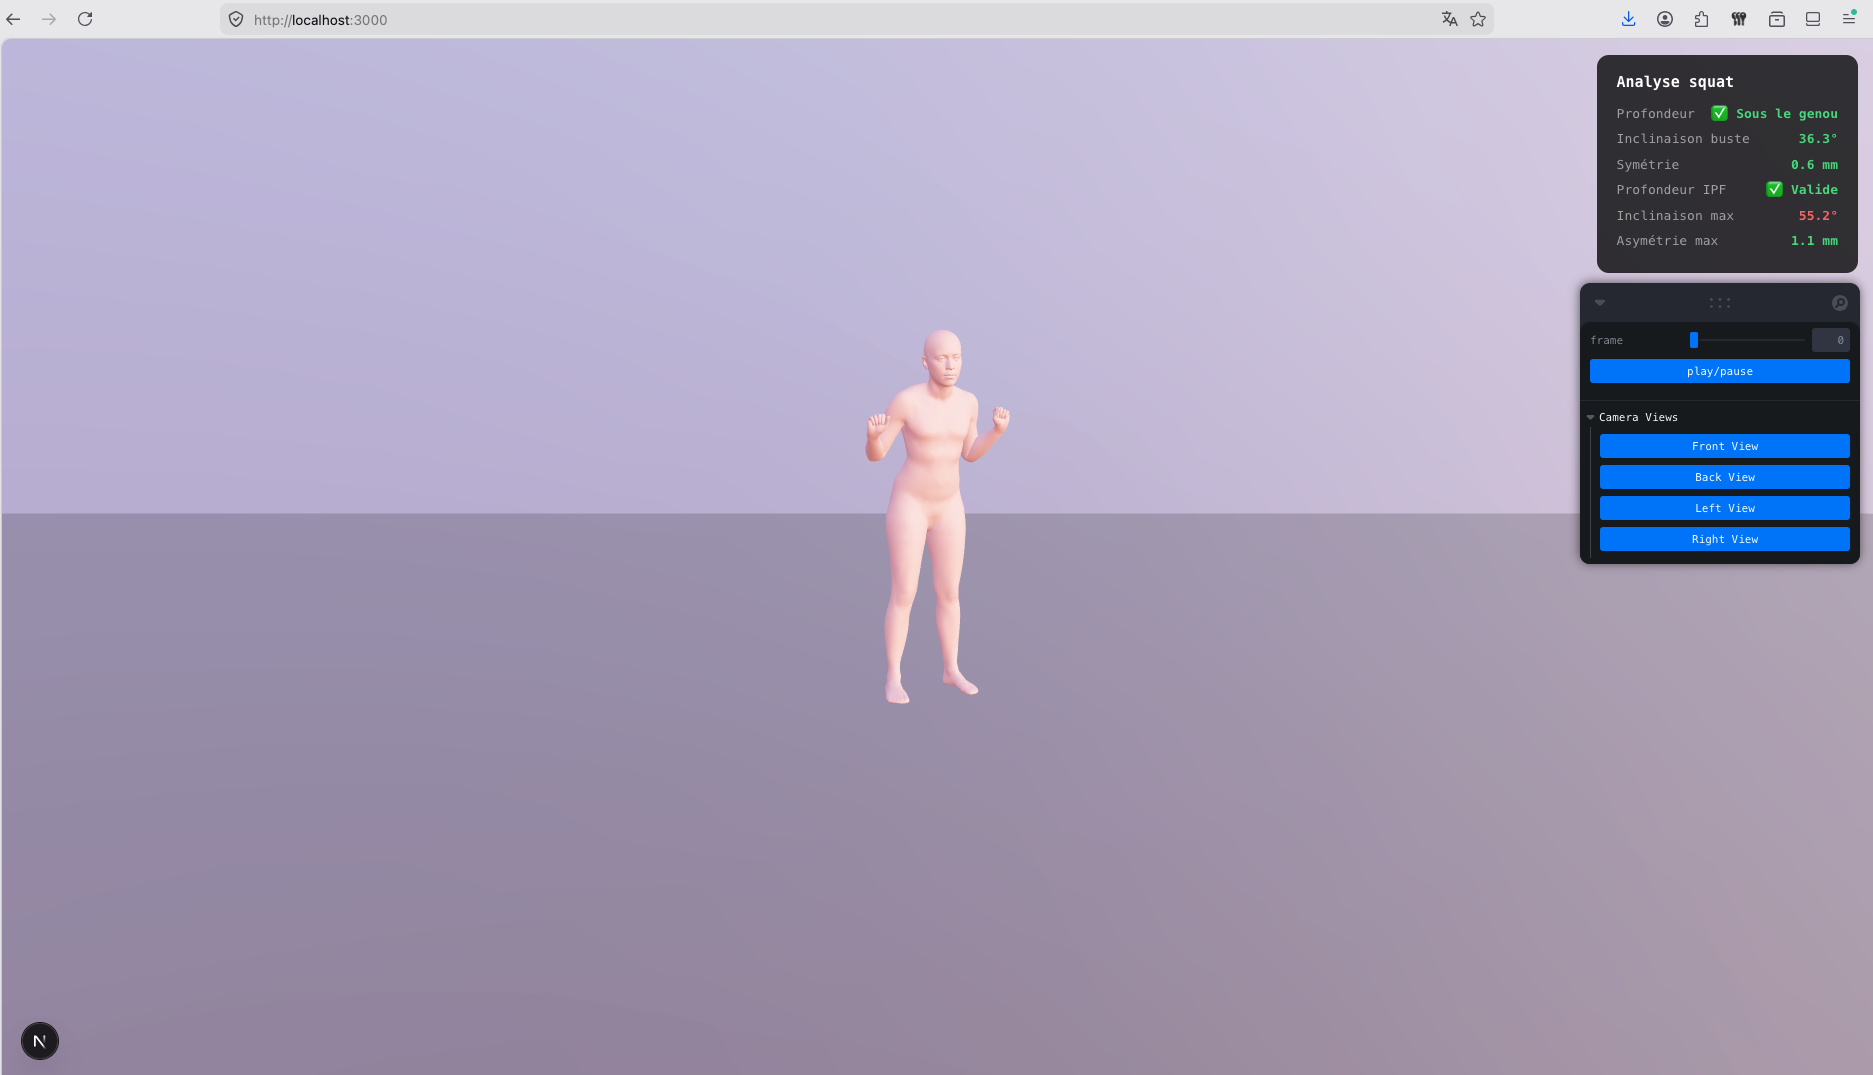
\includegraphics[width=5cm, height=3.5cm]{images/3-Pipeline_architecture/Squat-Web.png}
  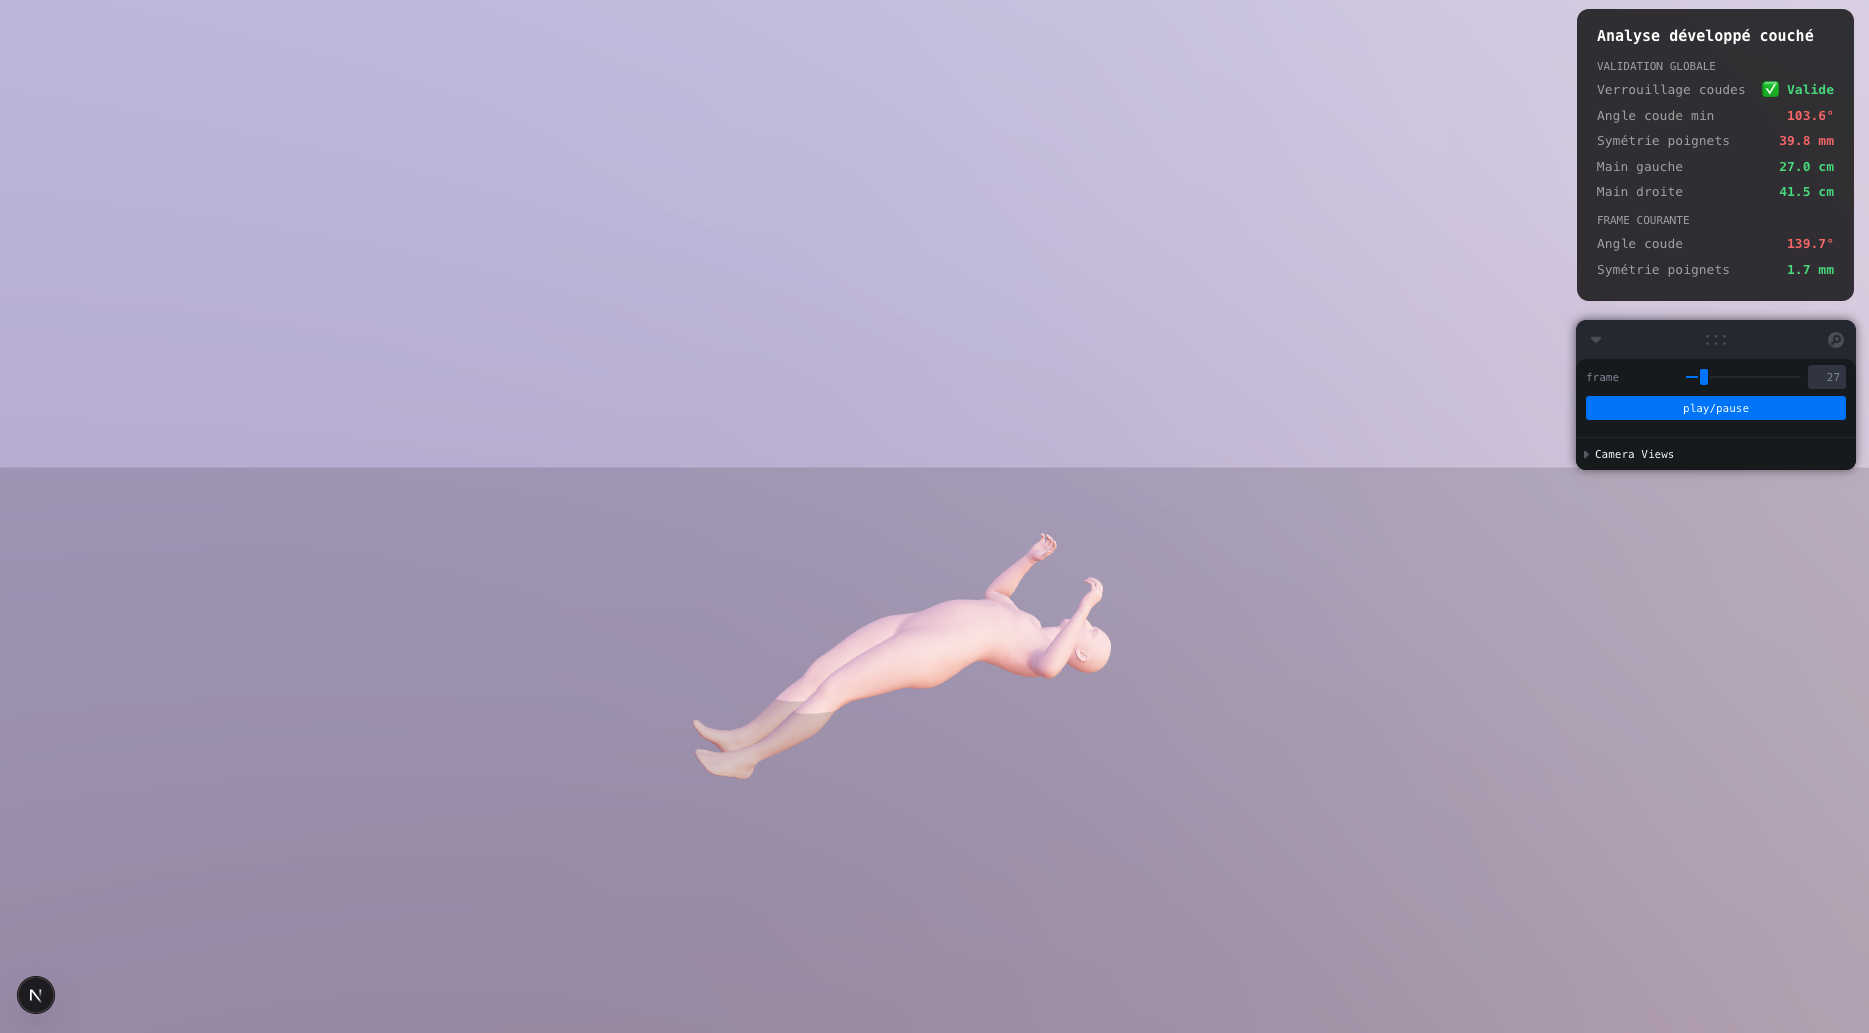
\includegraphics[width=5cm, height=3.5cm]{images/3-Pipeline_architecture/Bench-Web.png}
  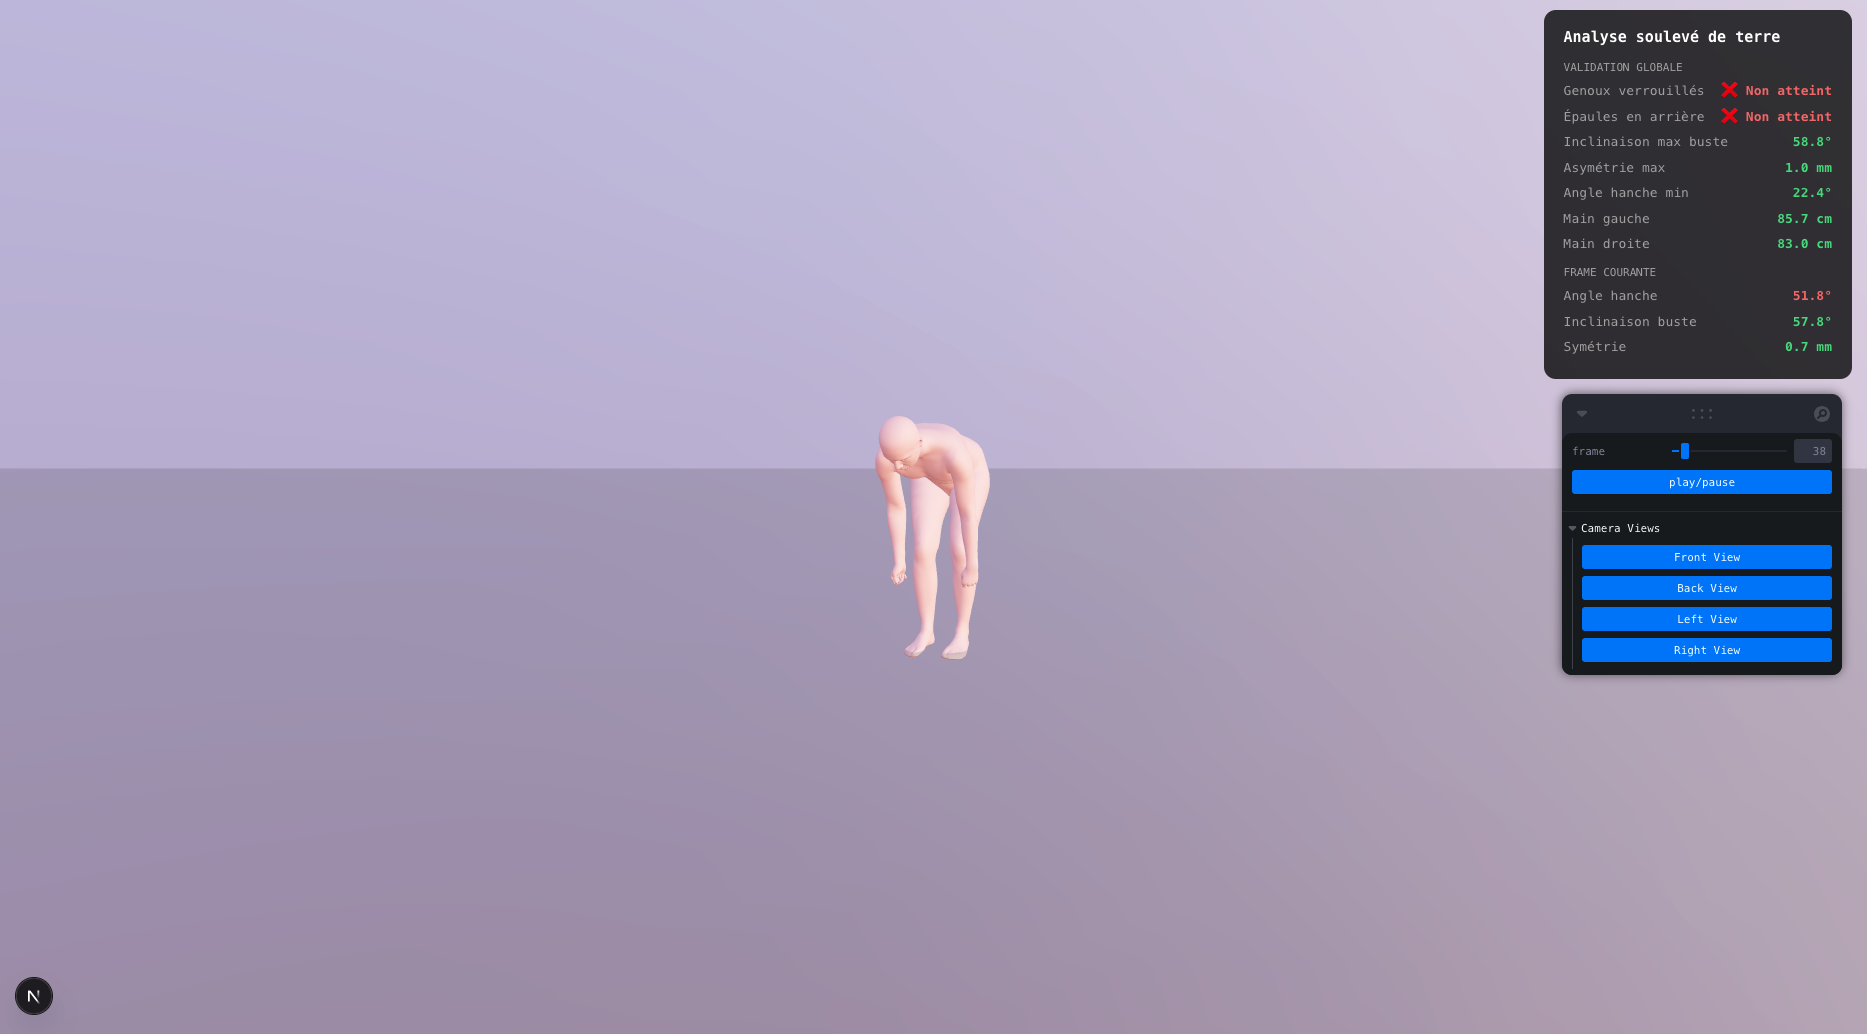
\includegraphics[width=5cm, height=3.5cm]{images/3-Pipeline_architecture/Deadlift-Web.png}
  \caption{Vue d'ensemble de l'application web de visualisation}
  \label{fig:web-visualisation}
\end{figure}

\subsection{Justification du choix}

Le HMR est un domaine compétitif où plusieurs modèles coexistent (PIXIE~\cite{PIXIE-2021}, HybrIK~\cite{HybrIK-2022}, HMR2.0~\cite{HMR-2-2023}, CLIFF~\cite{CLIFF-2022}, SMPLer-X~\cite{SMPLer-X-2024}, OSX~\cite{OSX-2023}, NLF~\cite{NLF-2024}, et SAM 3D Body~\cite{SAM-3D-Body-2026}). Le choix s'est porté sur 3DB pour les raisons suivantes :

\begin{itemize}
  \item \textbf{Performance en conditions réelles.} Les évaluations indépendantes et celles présentées par les auteurs placent 3DB en tête sur les benchmarks de poses inhabituelles et de conditions de prise de vue difficiles~\cite{SAM-3D-Body-2026}, ce qui correspond précisément aux poses extrêmes rencontrées en force athlètique.
  \item \textbf{Reconstruction full-body.} Contrairement à des modèles centrés sur le corps "simple" (SMPL~\cite{SMPL-2015}), 3DB inclut nativement les mains et les pieds, essentiels pour évaluer la prise sur la barre et l'appui au sol.
  \item \textbf{MHR.} Le découplage squelette/surface offert par MHR facilite l'analyse biomécanique : les indicateurs articulaires (angles, vitesses) peuvent être calculés directement sur le squelette sans interférence avec les variations de surface dues à l'habillement par exemple.
  \item \textbf{Open-source.} Le code et les checkpoints sont publiés en open-source, ce qui garantit la reproductibilité et permet un éventuel fine-tuning futur.
\end{itemize}

\subsection{Limites et alternatives}

Une limite principale doit être notée, 3DB opère image par image~\cite{SAM-3D-Body-2026} et ne garantit pas par construction la cohérence temporelle du maillage produit. 

Les alternatives écartées incluent :
\begin{itemize}
  \item HMR2.0 et CLIFF, plus rapides mais limités à SMPL (corps sans mains détaillées).
  \item SMPLer-X, corps entier mais moins robuste sur les poses extrêmes.
\end{itemize}

\section{Intégration et synchronisation des modules} \label{sec:integration}

\subsection{Gestion des dépendances et environnements}

Chaque modèle a été développé indépendamment par des équipes différentes, avec des dépendances Python parfois incompatibles (versions de PyTorch, CUDA, transformers, diffusers). Pour résoudre ce conflit, Pixi~\cite{Pixi-2024} a été utilisé comme gestionnaire d'environnements. Cet outil permet de créer un environnement isolé pour chaque module et de définir des pipelines d'exécution automatisant certaines tâches fastidieuses, notamment la construction du dataset.

\subsection{Synchronisation temporelle}

Les modules SAM3, MoGe-2 et SAM 3D Body opèrent trame par trame, produisant une sortie indépendante pour chaque image de la séquence. TACO, en revanche, requiert en entrée un clip vidéo de longueur fixe (14 trames consécutives dans la configuration retenue) et produit une séquence reconstruite de même longueur.

Pour traiter des séquences vidéo de longueur arbitraire avec TACO, une stratégie de fenêtre glissante sans chevauchement est appliquée : la séquence est découpée en clips de 14 trames consécutives et non recouvrantes. Lorsque la longueur totale de la séquence n'est pas un multiple de 14, la dernière fenêtre est décalée vers la gauche pour inclure les trames finales, créant un recouvrement minimal avec l'avant-dernière fenêtre. Les trames déjà reconstruites par la fenêtre précédente ne sont pas réécrites.

L'approche idéale consisterait à traiter la séquence entière en une seule passe, en fournissant à TACO l'intégralité des trames comme contexte temporel. Cela permettrait au modèle de tirer parti de la cohérence globale du mouvement pour guider la reconstruction des régions occluses. Cette approche se heurte toutefois aux limitations actuelles de la mémoire GPU : charger une séquence complète de plusieurs centaines de trames en mémoire vidéo reste hors de portée du matériel disponible. Le traitement par fenêtres de 14 trames constitue donc un compromis pratique, au prix d'une perte de contexte entre les fenêtres consécutives. Cette limite est identifiée comme une piste d'amélioration dans le chapitre~\ref{ch_six}.

\section{Choix techniques et justifications}

Au-delà du choix individuel des modèles, plusieurs décisions architecturales méritent d'être explicitées et sont détaillées dans cette section.

\subsection{Architecture séquentielle vs. bout-en-bout}

Une alternative aurait consisté à entraîner un unique modèle bout-en-bout, prenant en entrée une vidéo brute et produisant directement un maillage 3D animé. Cette approche a été écartée pour plusieurs raisons :

\begin{itemize}
  \item \textbf{Données d'entraînement.} Aucun dataset public ne fournit conjointement les annotations nécessaires (segmentation, profondeur métrique, complétion amodale, maillage 3D full-body) à l'échelle requise pour entraîner un tel système.
  \item \textbf{Coût.} L'entraînement d'un modèle multi-tâches de cette ampleur dépasserait largement les ressources et le temps disponibles dans le cadre de ce mémoire.
  \item \textbf{Modularité.} La rapide évolution de l'état de l'art rend hautement souhaitable la possibilité de remplacer un module sans réentraîner l'ensemble. Entre la planification du pipeline et sa finalisation, un des quatre modèles utilisés a reçu une mise à jour majeure (SAM3 $\to$ SAM 3.1~\cite{SAM3.1-2026}), introduisant une approche à mémoire partagée pour le suivi multi-objets, significativement plus rapide sans perte de précision.
\end{itemize}

\subsection{Inférence sur GPU} \label{sec:inference-sur-GPU}

L'ensemble du pipeline est conçu pour s'exécuter sur deux GPU NVIDIA RTX A5000. Cette contrainte a imposé un séquencement strict des modules avec libération de la mémoire GPU entre chaque étape.

\subsection{Choix du langage et du tramework}

L'ensemble du pipeline est implémenté en Python. Ce choix s'impose naturellement car tous les modèles sélectionnés étant distribués sous ce language. L'orchestration inter-modules est gérée par des scripts en Python pur.

\subsection{Versionnage des modèles et reproductibilité}

Chaque module est associé à un checkpoint figé, identifié par son empreinte cryptographique SHA-256. Les versions exactes utilisées dans ce mémoire sont consignées dans un fichier \texttt{models.lock} versionné avec le code source, garantissant la reproductibilité des résultats malgré les mises à jour fréquentes des modèles en amont. Les checkpoints eux-mêmes sont hébergés séparément et accessibles via les liens fournis dans le dossier \texttt{code/checkpoints} du dépôt.

Chaque module est associé à un checkpoint figé. Les versions exactes utilisées dans le mémoire sont consignées dans un fichier \texttt{models.lock} versionné avec le code source, garantissant la reproductibilité des résultats malgré les mises à jour fréquentes des modèles.

\medskip
Le pipeline défini ci-dessus constitue la base technique de la contribution principale de ce mémoire. Le chapitre suivant détaille la construction d'un dataset spécialisé et le protocole de \emph{fine-tuning} de TACO mis en place.